\chapter{Approach to certify Python Programs}
\label{ch:certify}
\subsection{ Category 1 constraint Generator : PC reset and fixed labels.}
\label{ch:c1}
This chapter describes working of first algorithm for constraint generation. All four algorithms are different because of different combination of PC label management scheme and  use of dynamic labels. In this algorithm we are using fixed label. Fixed label denotes that label will not change throughout the program. PC reset denotes that after completion of scope of a particular conditional/iteration body PC reset back to the PC just before the execution of conditional/iteration statement. PC monotonic denotes a scheme in which PC label never lose any information once it acquires, it just grows monotonically. This algorithm is able to capture basic information flows within a program, so this algorithm will certify a large number of programs as secure. Program certified secure by this algorithm does not mean that its fully secure, it certifies secure because of the limitation in detection of information flows in program. Some information flows which are not captured by this algorithm may violate information security.\\
\subsection{Working}
All four algorithm shares same basic structure for parsing input program. Dynamic analysis can not process all branches in a one go but static analysis process all branches in one run. Algorithms generates constraints for all possible control branches in program.  PC keeps track of variables used in conditional statement and iteration statement. Assignment operation are responsible for information flows so at each occurrence of assignment operation constraints generated with the help of PC label.
\section{Constraint Rules}
\begin{enumerate}
	\item < x := e > generate constraint [$\lambda(e)\oplus\lambda(PC)\le\lambda(x)$] and update PC label\\ $\lambda(PC) = \lambda(e)\oplus\lambda(PC)$ 
	\item < x := e > generate constraint [$\lambda(e)\oplus\lambda(PC)\le\lambda(x)$] and update PC label\\ $\lambda(PC) = \lambda(e)\oplus\lambda(PC)$ 
	\item < if e then c1 else c2>  $\forall  x \in ( modified\_global(\hspace{0.2cm} c1 \hspace{0.2cm}and \hspace{0.2cm} c2) \cup \{PC\} )$ generate constraints [$\lambda(e)\oplus\lambda(PC)\le\lambda(x)$] and update PC label $\lambda(PC) = \lambda(e)\oplus\lambda(PC)$
	
	\item < while e do c > $\forall  x \in ( modified\_global(c) \cup \{PC\} )$ generate constraints [$\lambda(e)\oplus\lambda(PC)\le\lambda(x)$] and update PC label $\lambda(PC) = \lambda(e)\oplus\lambda(PC)$
\end{enumerate}

\begin{figure}
	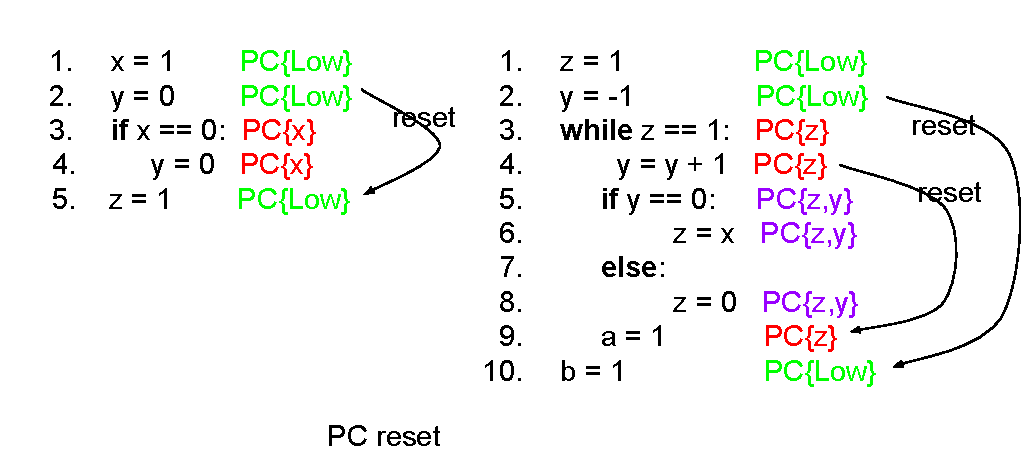
\includegraphics[width=1\textwidth]{PC_reset.pdf}
	\centering
	\caption{Example for PC reset}
	\label{fig:pcreset}
\end{figure}
\begin{figure}
	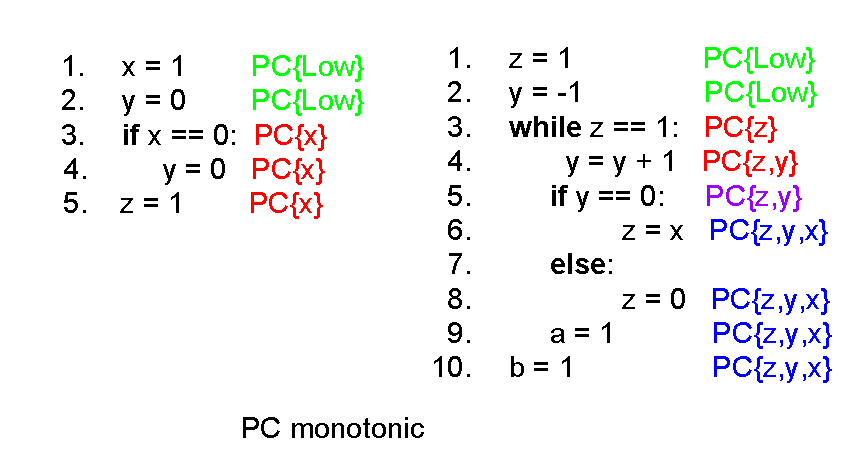
\includegraphics[width=1\textwidth]{PC_monotonic.pdf}
	\centering
	\caption{Example for PC monotonic}
	\label{fig:pcreset}
\end{figure}
\subsection{Key Idea}
Direct information flow happens because of copying or assigning values. Implicit information flow happens because of control dependency, this algorithm focuses on information flow from variables used in condition statement of if else(conditional)
and while(iteration) to all variables modified in the body of iteration or conditional.
\begin{lstlisting}[language=Python,caption={Python example}, label={lst:p1copy1}]
def(x,y):     #copy x to y
y = 0
z = 0
if x == 0:    # implicit flow x -> z PC{x}
z = 1
if z == 0:    # implicit flow z-> y PC{z}
y = 1
p = q         # direct flow q -> p PC{q}
\end{lstlisting}
Constraints generated by this algorithm for listing \ref{lst:p1copy1} are given below. 
\begin{itemize}
	\item x <= z
	\item z <= y
\end{itemize}
\section{Limitations}
For listing \ref{lst:p1copy1} this algorithm is able to capture all information flows, but in more complex programs it may declare falsely a program secure.
\begin{lstlisting}[language=Python, caption=Python version of copy5 example in \cite{denning}. goal: information flow from x to y, label={lst:p1copy5} ]
#Procedure copy5
y = 0
while x==0 :
pass
y = 1
\end{lstlisting}
For listing \ref{lst:p1copy5} this algorithm generated only one constraint Low <= y, that shows this algorithm will certify listing \ref{lst:p1copy5} secure always irrespective of information flow x to y is secure or not. All these limitation in capturing information flow raised because of PC label management in this algorithm is only focus on local information flow. Next algorithm will try to remove these limitation using monotonic PC label management. Appendix A shows the implementation of this algorithm.
\begin{lstlisting}[language=Python, caption=Python version of dynamic label example in \cite{denning}. goal: information flow from x to y, label={lst:p1dynamic} ]
def fun(x, y, z):
a = x
y = a
a = z
fun(x, y, z)
\end{lstlisting}
Another limitation of this algorithm is related to use of fixed label. In listing \ref{lst:p1dynamic} this algorithm detect false information flow z to y. Category 3 uses both dynamic and fixed label to remove this limitation.
\section{Category 2 constraints : PC monotonic and fixed labels.}
This chapter describes working of category 2 constraint generator. This algorithm is a improved version of previous category 1 algorithm. This algorithm using monotonic PC label instead of PC reset. By using monotonic PC this algorithm is able to detect additional information flows in program.
\subsection{Working}
rules
\subsection{Key Idea}
This analysis extension of previous algorithm, non terminating loops
create a control dependency between variables used in condition of loop and
the rest of the code where control can go subsequently on termination of loop,
because of this behavior of non terminating loop PC storing all the dependencies.

\subsection{Limitations}  
In static analysis if constraint resolver ignores the order of generated constraints then it may show some additional false information flow in program, this is responsible for overhead and imprecision in certification process. Use of dynamic label solves this problem easily on the cost of more complex analysis.
\begin{lstlisting}[language=Python, caption=Python version of dynamic label example in \cite{denning}. goal: information flow from x to y, label={lst:p2dynamic} ]
def fun(x, y, z):
a = x
y = a
a = z
fun(x, y, z)
\end{lstlisting}
constraints generated for listing \ref{lst:p2dynamic} are given below:
\begin{itemize}
	\item x <= a
	\item a + x <= y
	\item a + x + z <= a
\end{itemize}
these constraints shows that there is information flow z to y ( using a <= y and z <= a) but in program there is no such flow exist. Because of such information flow constraint resolver may certify a secure program as not secure and it also create extra overhead on resolver. This example shows flaw in approach of using fixed label everywhere. Next algorithm will try to remove this limitation.
\section{Category 3 constraints : PC reset and dynamic labels.}
\label{ch:c3}
This chapter describes category 3 constraint generator. This algorithm introduces use of dynamic label. Global variable are using fixed label and all local variables are assigned dynamic label. Information can flow outside only because of modification of global variable, modification of local variable doe not cause information because information remains in program itself.   
\subsection{Constraint Rules}
\begin{itemize}
	\item < x := e > generate constraint [$\lambda(e)\oplus\lambda(PC)\le\lambda(x)$] and update PC label\\ $\lambda(PC) = \lambda(e)\oplus\lambda(PC)$ 
	\item < if e then c1 else c2> \begin{enumerate}
		\item $\forall  x \in ( modified\_global(\hspace{0.2cm} c1 \hspace{0.2cm}and \hspace{0.2cm} c2) \cup \{PC\} )$ generate constraints [$\lambda(e)\oplus\lambda(PC)\le\lambda(x)$] and update PC label $\lambda(PC) = \lambda(e)\oplus\lambda(PC)$
		\item $\forall x \in ( modified\_local(\hspace{0.2cm} c1 \hspace{0.2cm}and \hspace{0.2cm} c2) \cup \{PC\} )$ update PC label $\lambda(PC) = \lambda(e)\oplus\lambda(PC)$
	\end{enumerate}
	\item < while e do c > \begin{enumerate}
		\item $\forall  x \in ( modified\_global(c) \cup \{PC\} )$ generate constraints [$\lambda(e)\oplus\lambda(PC)\le\lambda(x)$] and update PC label $\lambda(PC) = \lambda(e)\oplus\lambda(PC)$
		\item $\forall x \in ( modified\_local(c) \cup \{PC\} )$ update PC label $\lambda(PC) = \lambda(e)\oplus\lambda(PC)$
	\end{enumerate}
\end{itemize} 
In static analysis if constraint resolver ignores the order of generated constraints then it may show some additional false information flow in program, this is responsible for overhead and imprecision in certification process.
Use of dynamic label solves this problem easily on the cost of more complex analysis.\\~\\
'a' is a local variable in function defined below.\\
def function(x,y,z):\\
\hspace*{1cm}a = x\\
\hspace*{1cm}y = a\\
\hspace*{1cm}a = z\\~\\
static analysis will generate constraints 1. x$\le$a, 2. a$\le$y, 3. z$\le$a.\\
Last two constraints shows false information flow from z to y (z\marr y).\\~\\
Dynamic label analysis\\
1. $\lambda(a)$ := x\\
2. $y\le \lambda(a) \{x\}$\\
3. $\lambda(a) := z $\\~\\
This analysis treats global and local variable differently so it avoids false constraints successfully without tracking order of constraints explicitly.\\~\\
a = x\\
while 1:\\
\hspace*{1cm} y = a\\
\hspace*{1cm} a = z\\~\\
Dynamic label Analysis:\\
First iteration of while:\\
1. $\lambda(a)$ := x\\
2. $y\le \lambda(a) \{x\}$\\
3. $\lambda(a) := z $\\~\\
Second Iteration:\\
2. $y\le \lambda(a) \{z\}$\\
3. $\lambda(a) := z $\\~\\
Dynamic label analysis generating different constraints for first iteration and second iteration but static analysis is not able to distinguish between information flow in first iteration and second iteration of while loop.
\subsection{Key Idea}
Definition of information flow among objects : If any data can be
guessed by using given objects which was unknown previously, by using this
idea information can flow outside only because of modification of global objects,
so any information flow from local objects to global objects must be
checked for security breach. Local variable plays a role of temporary in flow
of information from one global to another, so local variable must keep track
of information they hold, dynamic label is a good technique to keep track of
history of information stored in a local variable.
\subsection{Limitations}
This constraint generator again using PC reset label scheme. We created this category for thorough analysis and comparison among all categories. So it shares the first limitation of category 1. It fails to capture global information flows created by non terminating loops.   
\section{Category 4 constraints: PC monotonic and dynamic label.}
\label{ch:c4}
This algorithm is best among all four algorithm in terms information security. Dynamic label processing increases time complexity of this algorithm but we used a property of PC label to make optimization.
Constraint generation rules are same as category 3.
\subsection{Key Idea} In this analysis PC never gets reset because we want to track all possible information flows including information flows from a nonterminating loop to rest of code.\\ 
'a' is a local var\\
a = x\\
while w:\\
\hspace*{1cm} y = a\\
\hspace*{1cm} a = z\\
z = y\\~\\
Dynamic label Analysis:\\
1. $\lambda(a) = x$\\
2.PC\{w\}\\
3.PC\{w, $\lambda$(a)\{x\}\} \hspace{1cm} $w\oplus x \le y$\\
4.$\lambda(a) = z$\\
5.PC\{w, x, y\} \hspace{1cm} $w\oplus x\oplus y \le z$\\

So this algorithm is capable to track information flow w\marr z in last statement z = y by using monotonic PC without generating additional false constraints. 
\subsection{Limitations}
Use of dynamic label with monotonic creates challenge for processing of large number of labels.  
\section{Comparison among all categories of constraints.}
\label{ch:comp}
\begin{table}
	\hspace{-2cm}
	\begin{tabular}{|l|l|l|l|l|}
		\hline
		Input Program  &  C1 & C2 & C3 & C4 \\
		\hline
		\begin{lstlisting}[language=Python]
		#'a' is a local var
		a = x
		while w:
		y = a
		a = z
		z = y
		\end{lstlisting}&
		\begin{lstlisting}
		x <= a
		a + w <= y
		z + w <= a
		y <= z
		\end{lstlisting}&
		\begin{lstlisting}
		x <= a
		a + x + w <= y
		a + x + z + w <= a
		a + x + z + w <= y
		a + x + z + y + w <= z
		y + x + w <= z
		\end{lstlisting}&
		\begin{lstlisting}
		x + w <= y
		x + z + w <= y
		y <= z	
		\end{lstlisting}&
		\begin{lstlisting}
		x + w <= y
		x + z + w <= y
		y + x + w <= z
		y + x + z + w <= z	
		\end{lstlisting}\\
		\hline
		
	\end{tabular}
	\caption{Example for comparison}
	\label{tbl:compex}
\end{table}


Example given in table \ref{tbl:compex} is suitable to differentiate between all category.
First algorithm fails to track information flow w\marr z in last statement z = y.
Second algorithm is able to track information flow w\marr z in last statement z = y but it will show additional false information flow z \marr y too. 
Third algorithm avoids tracking of additional false information flow z \marr y but it fails to show information flow w \marr z because of PC reset.
Fourth analysis avoids tracking of false information flow as well as tracks information flow caused by nonterminating loop( w \marr z). Table \ref{tbl:compcopy} shows constraints generated for copy program given in Denning,s book by all constraint generator.
\begin{table}
	\hspace{-2cm}
	\begin{tabular}{|l|l|l|l|l|}
		\hline
		Programs  &  C1 & C2 & C3 & C4 \\
		\hline
		Copy1&
		\begin{lstlisting}
		x <= z
		z <= y
		\end{lstlisting}&
		\begin{lstlisting}
		x <= z
		x + z <= y
		\end{lstlisting}&
		\begin{lstlisting}
		x <= y
		\end{lstlisting}&
		\begin{lstlisting}
		x <= y
		\end{lstlisting}\\
		\hline
		Copy2&
		\begin{lstlisting}
		Low <= z
		Low <= y
		y + z <= y
		y + x + z <= z
		y + z <= z
		\end{lstlisting}&
		\begin{lstlisting}
		Low <= z
		Low <= y
		y + z <= y
		y + x + z <= z
		y + z <= z
		y + x + z <= y
		\end{lstlisting}&
		\begin{lstlisting}
		Low <= y
		y <= y
		y + x <= y
		\end{lstlisting}&
		\begin{lstlisting}
		Low <= y
		y <= y
		y + x <= y
		\end{lstlisting}
		\\
		\hline
		Copy3&
		\begin{lstlisting}
		x + s0 <= s0
		x + s1 <= s1
		s0 <= s0
		Low <= y
		s1 <= s1
		\end{lstlisting}&
		\begin{lstlisting}
		x + s0 <= s0
		x + s1 <= s1
		s0 <= s0
		s0 <= y
		s1 + s0 <= s1
		s1 <= s1
		s1 <= y
		s1 + s0 <= s0
		\end{lstlisting}&
		\begin{lstlisting}
		x + s0 <= s0
		x + s1 <= s1
		s0 <= s0
		Low <= y
		s1 <= s1
		\end{lstlisting}&
		\begin{lstlisting}
		x + s0 <= s0
		x + s1 <= s1
		s0 <= s0
		s0 <= y
		s1 + s0 <= s1
		s1 <= s1
		s1 <= y
		s1 + s0 <= s0
		\end{lstlisting}
		\\
		\hline
		Copy4&
		\begin{lstlisting}
		x <= e0
		x <= e1
		Low <= y
		Low <= e1
		Low <= e0
		\end{lstlisting}&
		\begin{lstlisting}
		x <= e0
		x <= e1
		e0 <= y
		e0 <= e1
		e1 <= y
		e1 <= e0
		\end{lstlisting}&
		\begin{lstlisting}
		x <= e0
		x <= e1
		Low <= y
		Low <= e1
		Low <= e0
		\end{lstlisting}&
		\begin{lstlisting}
		x <= e0
		x <= e1
		e0 <= y
		e0 <= e1
		e1 <= y
		e1 <= e0
		\end{lstlisting}
		\\
		\hline
		Copy5&
		\begin{lstlisting}
		Low <= y
		\end{lstlisting} &
		\begin{lstlisting}
		Low <= y
		x <= y
		\end{lstlisting}&
		\begin{lstlisting}
		Low <= y 
		\end{lstlisting}&
		\begin{lstlisting}
		Low <= y
		x <= y
		\end{lstlisting}\\
		\hline
		Copy6&
		\begin{lstlisting}
		Low <= z
		Low <= sum
		Low <= y
		x + sum + z <= sum
		y + z <= y
		\end{lstlisting}&
		\begin{lstlisting}
		Low <= z
		Low <= sum
		Low <= y
		x + sum + z <= sum
		y + x + sum + z <= y
		y + x + sum + z <= sum
		\end{lstlisting} &
		\begin{lstlisting}
		Low <= y
		y <= y  
		\end{lstlisting}&
		\begin{lstlisting}
		Low <= y
		y + x <= y
		\end{lstlisting}\\
		\hline
		Dynamic label&
		\begin{lstlisting}
		x <= a
		a <= y
		z <= a
		\end{lstlisting}&
		\begin{lstlisting}
		x <= a
		a + x <= y
		a + x + z <= a
		\end{lstlisting} &
		\begin{lstlisting}
		x <= y
		\end{lstlisting}&
		\begin{lstlisting}
		x <= y
		\end{lstlisting}\\
		\hline
	\end{tabular}
	\label{tbl:compcopy}
	\caption{Constraints generated by all four algorithm for copy programs given Denning \cite{denning}}
\end{table}
\begin{figure*}[h]
	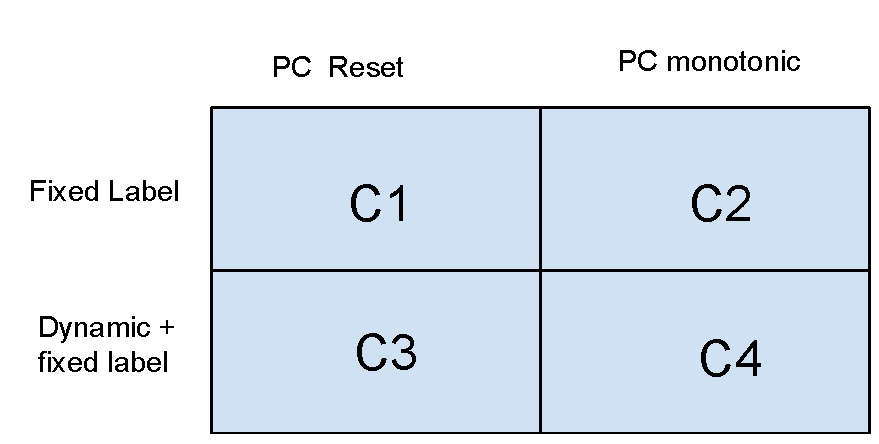
\includegraphics[width=0.6\textwidth]{category}
	\centering
	\caption{Category of constraint generator}
	\label{fig:set}
\end{figure*}
\begin{figure*}[h]
	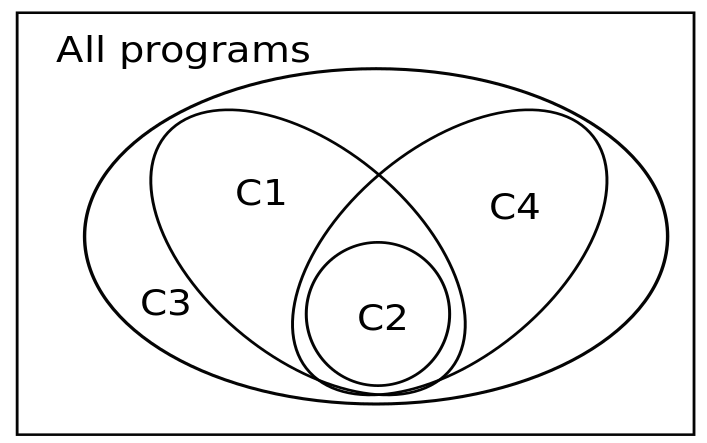
\includegraphics[width=0.6\textwidth]{rsz_set}
	\centering
	\caption{Set diagram}
	\label{fig:set}
\end{figure*}
Figure \ref{fig:set} shows the relationship between set of programs declared secure by all constraint generator. C1-C4 are abbreviation for category 1 - category 4. Number of constraints is inversely proportional to size of set of program declared secure, because more constraints means high probability of violation of security. In category 1 generator generates many false constraints because of absence of dynamic label, but category 3 uses dynamic labels with fixed so it reduces number of constraints. Constraints generated by category 1 are superset of constraints generated by category 3 this relationship shows that set of program declared secure by C1 must be subset of C3. Similarly C2 and C4 differ by use of dynamic labels so set of accepted program by C2 is a subset of set of programs accepted by C4. Use of monotonic PC label helps to capture global information flows so use of monotonic PC label increases the number of constraints. C3 and C4 differ by use of PC label scheme, C4 using monotonic PC and C3 using PC reset so constraints generated by C4 are superset of constraints generated by C3 so set of accepted programs of C4 must be subset of C3. Similarly C2 and C1 differ by PC label scheme so set of accepted programs is a subset of set of programs accepted by C1.    
\begin{figure}
	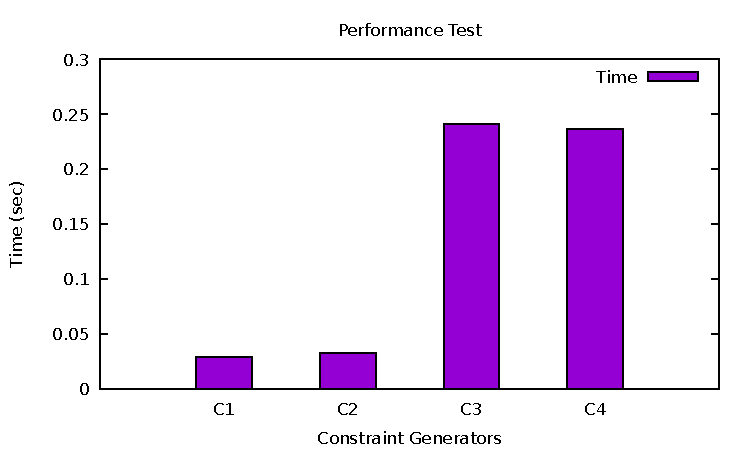
\includegraphics[width=1\textwidth]{graph.pdf}
	\centering
	\caption{Performance test}
	\label{fig:ptest}
\end{figure}
Figure \ref{fig:ptest} shows the average time taken in processing one copy program by all four generator. 
Time taken in order C1 < C2 < C4 < C3. C4 taking little less time than C3 because of optimization in label generation, this optimization uses property of monotonic PC so it can not applied in C3.
